\begin{IEEEbiography}[{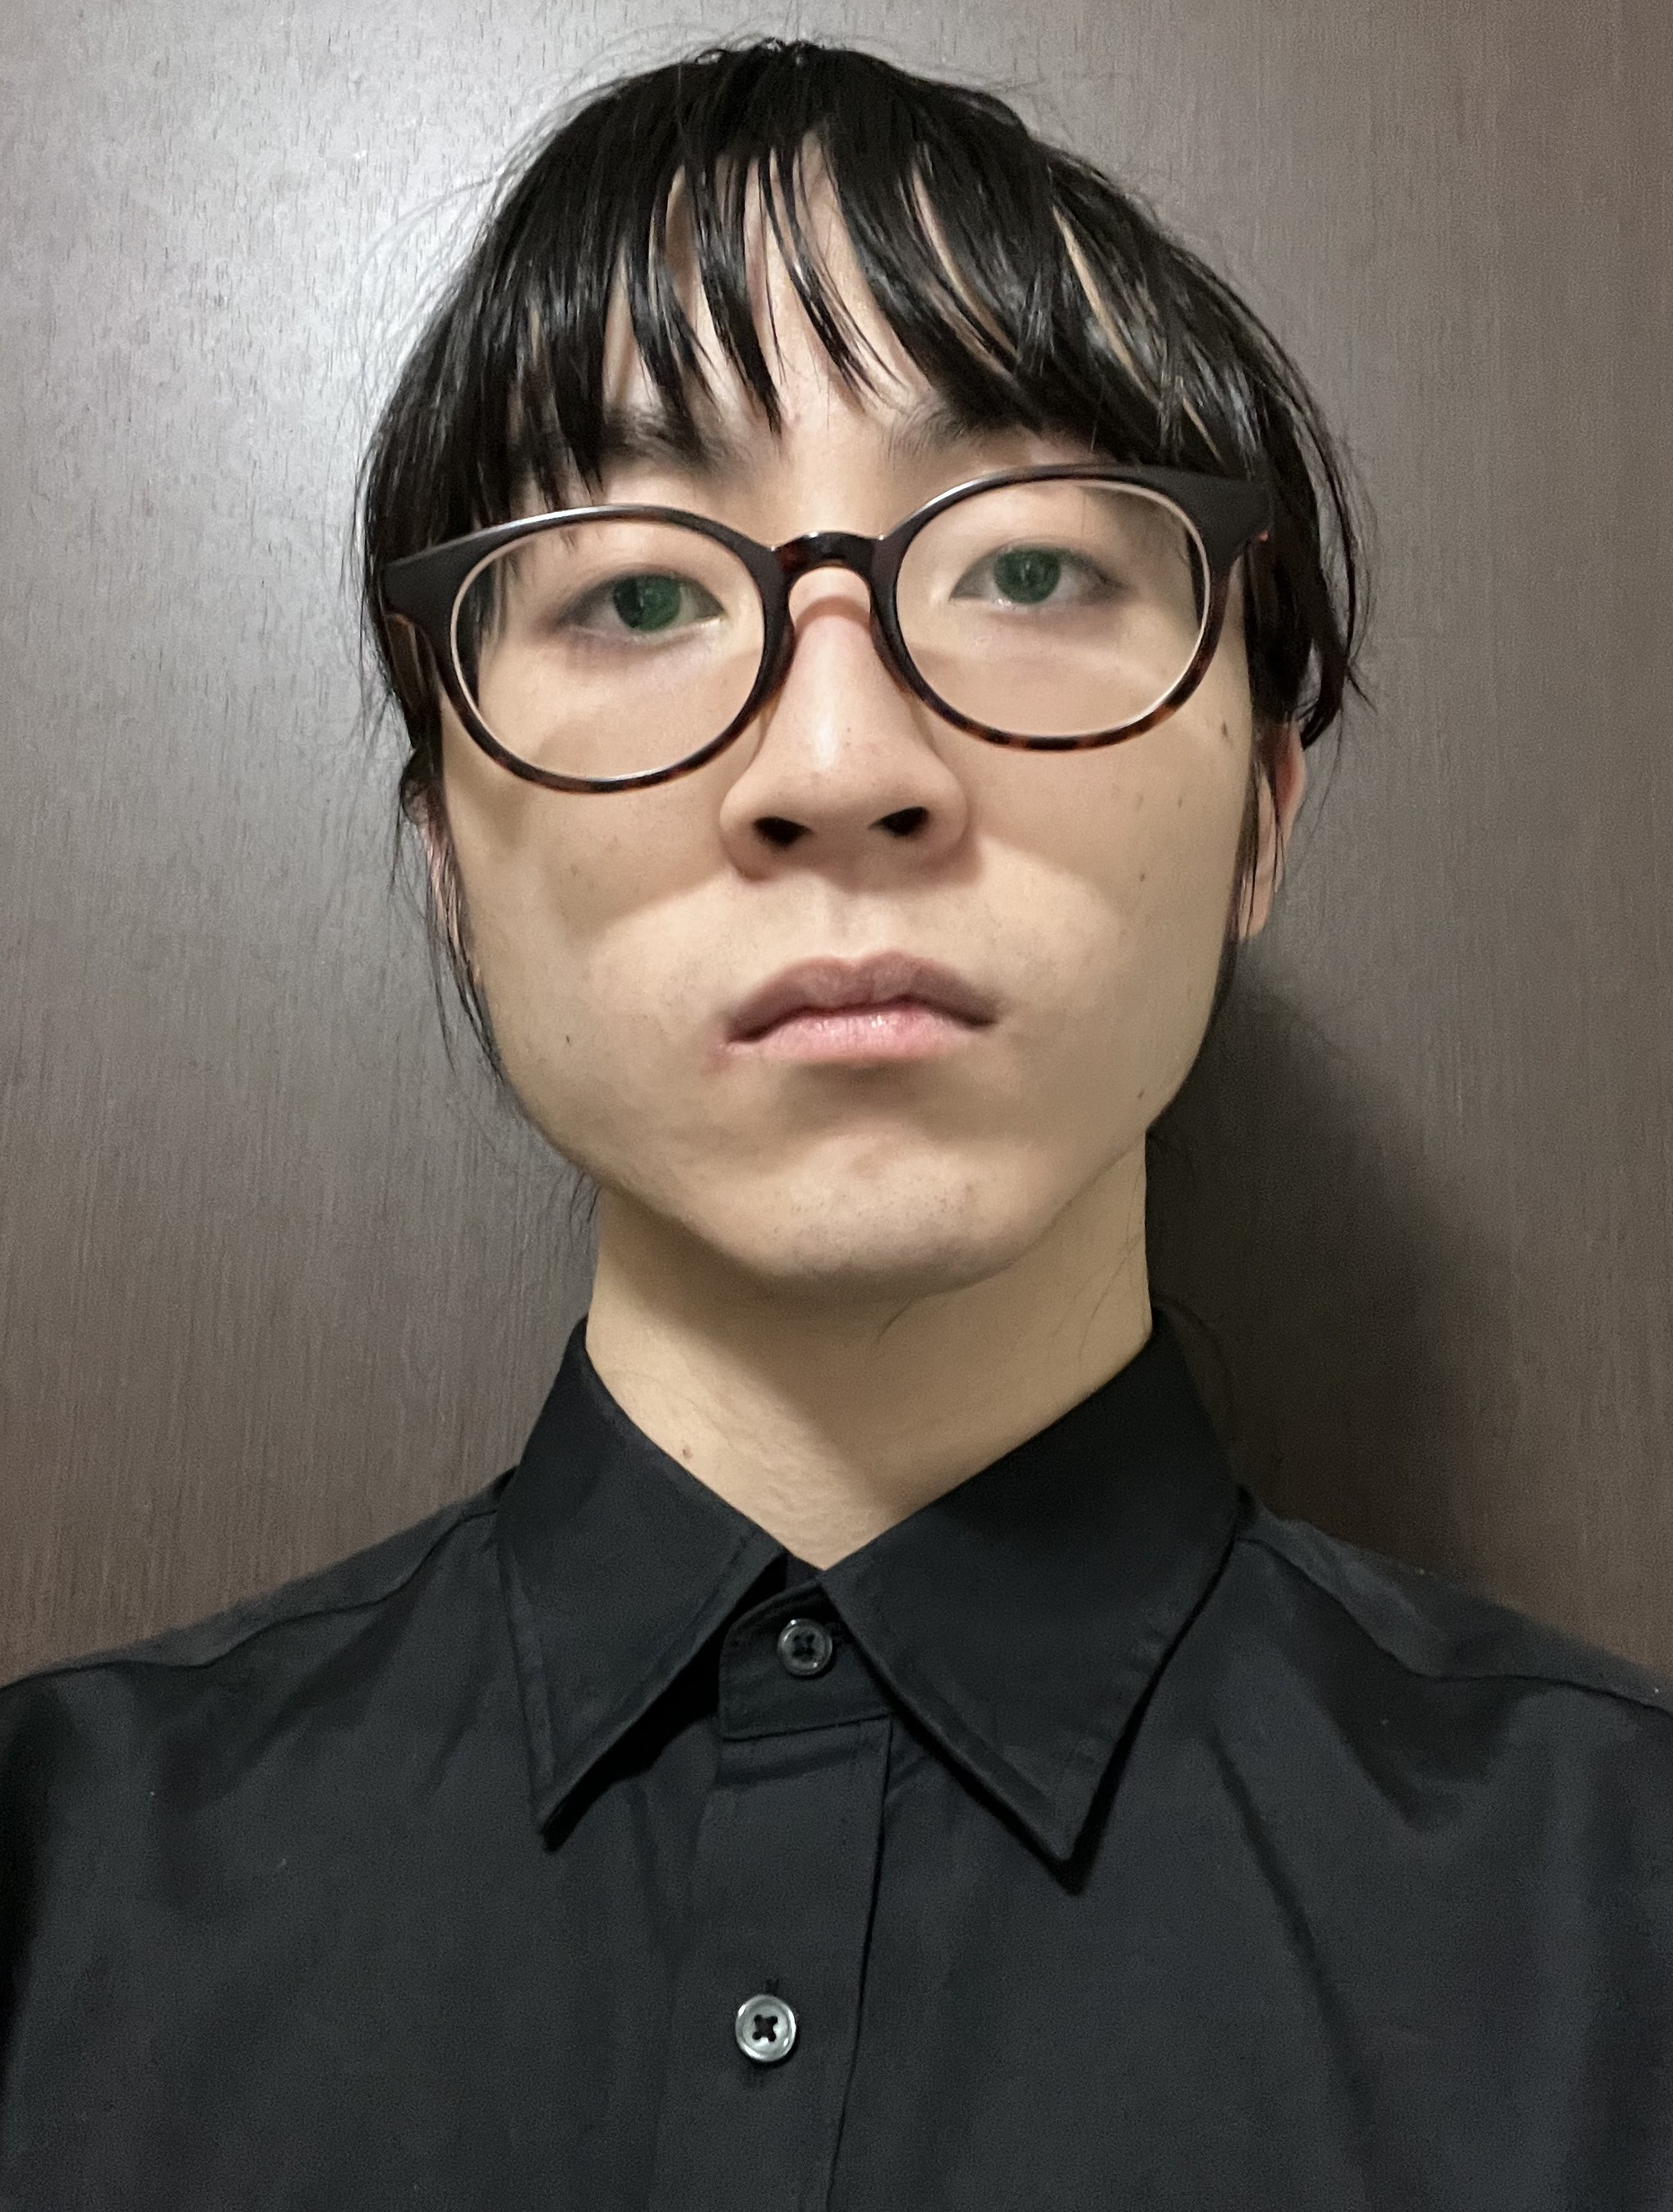
\includegraphics[width=1in,height=1.25in,clip,keepaspectratio]{img/sano2.jpg}}]{Wataru Sano} received the B.E. degree from the Undergraduate School of Computer Science and Engineering, Shibaura Institute of Technology, Tokyo, Japan, in 2024. He is currently pursuing the M.E. degree with the Graduate School of Electric Engineering and Computer Science, Shibaura Institute of Technology. 
\end{IEEEbiography}

\begin{IEEEbiography}[{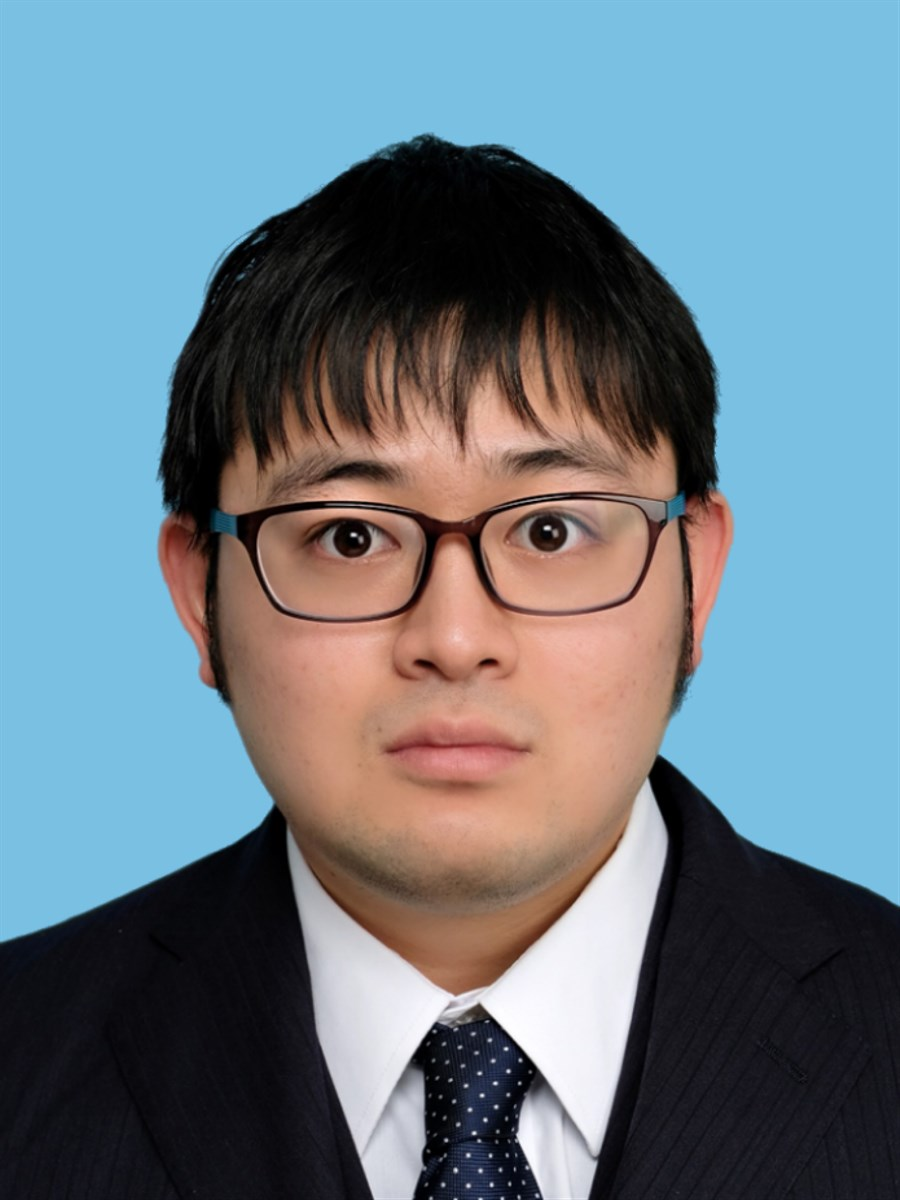
\includegraphics[width=1in,height=1.25in,clip,keepaspectratio]{img/Watanabe.jpg}}]{Jumpei Watanabe} received the B.E. degree from the Undergraduate School of Computer Science and Engineering, Shibaura Institute of Technology, Tokyo, Japan, in 2023.
He received the M.E. degree from the Graduate School of Electrical Engineering and Computer Science, Shibaura Institute of Technology, Tokyo, Japan, in 2025.
\end{IEEEbiography}
  
\begin{IEEEbiography}[{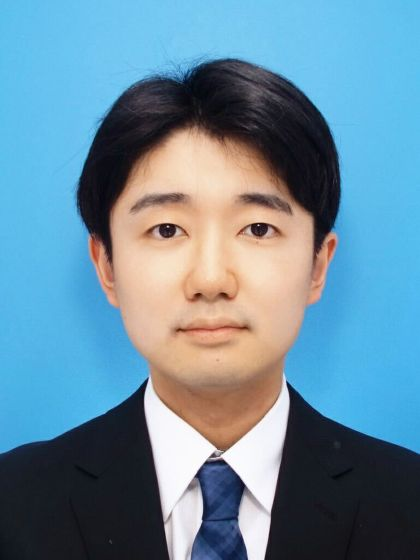
\includegraphics[width=1in,height=1.25in,clip,keepaspectratio]{img/pic_2025.jpg}}]{Haruma Shiraishi}
received the B.E. degree from the
Undergraduate School of Computer Science and Engineering, Shibaura Institute of Technology, Tokyo,
Japan, in 2025. He is currently pursuing the M.E. degree with the Graduate School of Electric Engineering and Computer Science, Shibaura Institute of Technology.
\end{IEEEbiography}

\begin{IEEEbiography}[{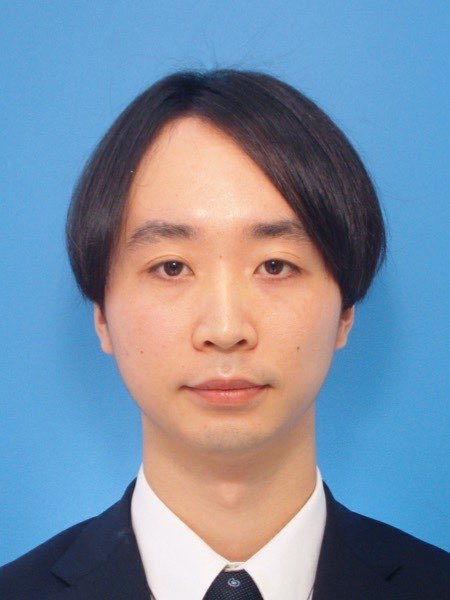
\includegraphics[width=1in,height=1.25in,clip,keepaspectratio]{img/rsugano.jpg}}]{Ryusei Sugano} (Graduate Student Member, IEEE) 
received the M.E. degree with the Graduate School of Electric Engineering and Computer Science, Shibaura Institute of Technology.
He is currently pursuing the Ph.D. degree with the Graduate School of Electric Engineering and Computer Science, Shibaura Institute of Technology.
\end{IEEEbiography}

\begin{IEEEbiography}[{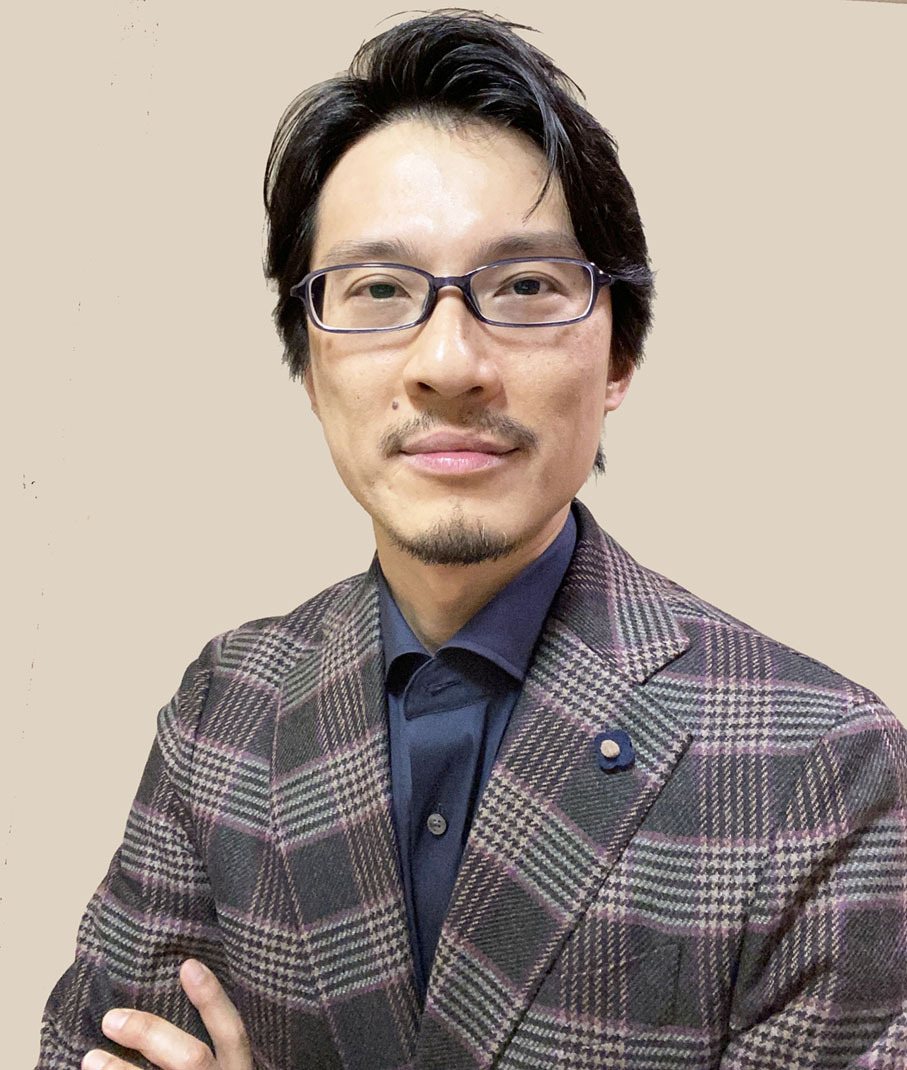
\includegraphics[width=1in,height=1.25in,clip,keepaspectratio]{img/RShinkuma.jpg}}]{Ryoichi Shinkuma} (Senior Member, IEEE) 
received the B.E., M.E., and Ph.D. degrees in communications engineering from Osaka University, Suita, Osaka, Japan, in 2000, 2001, and 2003, respectively. 
He joined the Graduate School of Informatics, Kyoto University, Kyoto, Japan, where he has worked as an Assistant Professor from 2003 to 2011 and an Associate Professor from 2011 to 2021. 
He was a Visiting Scholar with the Wireless Information Network Laboratory, Rutgers University, New Brunswick, NJ, USA, from 2008 to 2009.
In 2021, he joined the Faculty of Engineering, Shibaura Institute of Technology, Tokyo, Japan, as a Professor. 
In May 2022, he founded Hyper Digital Twins (HDT) Company Ltd., Tokyo, where he is currently the CTO. 
\end{IEEEbiography}

\begin{IEEEbiography}[{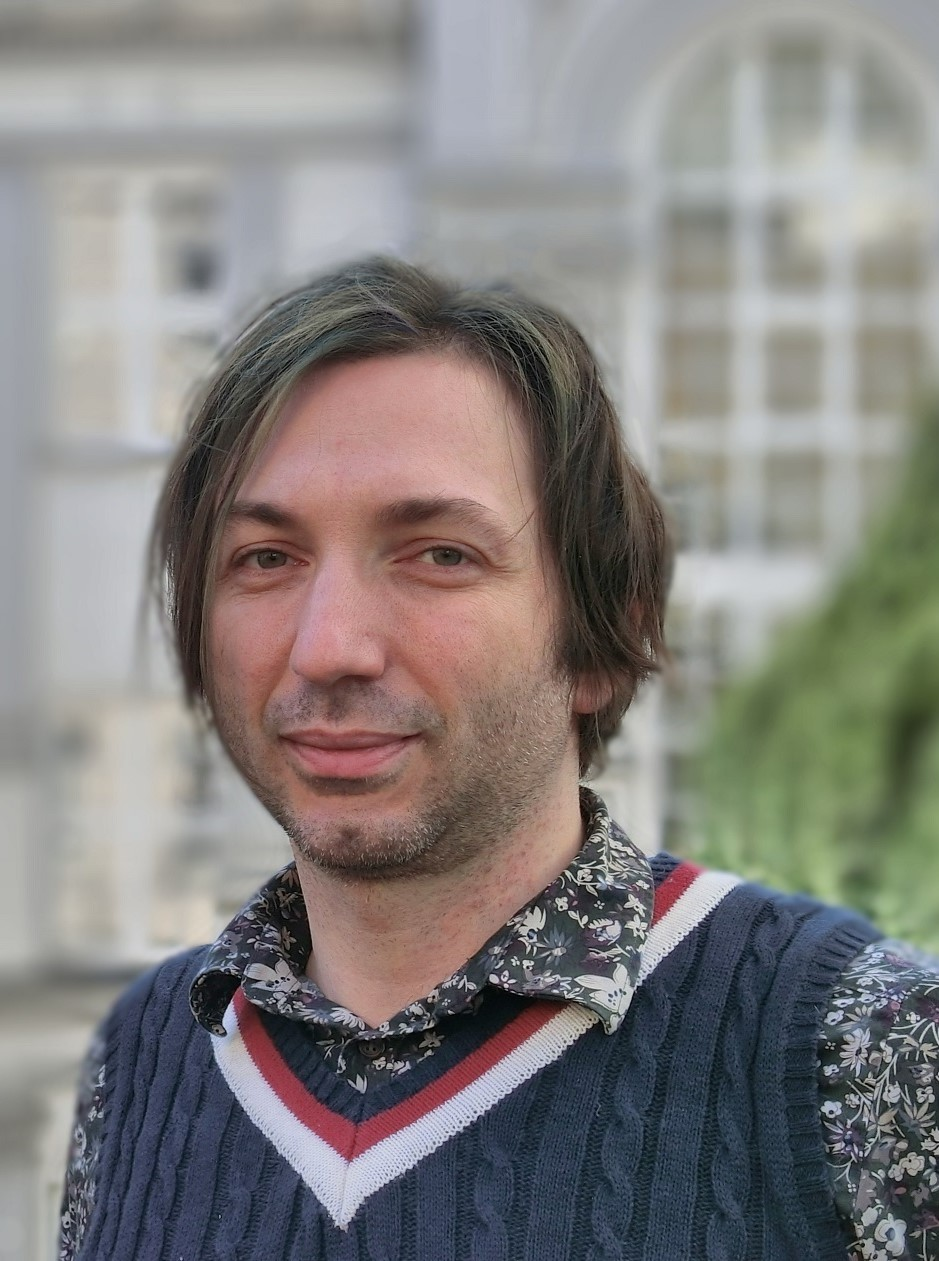
\includegraphics[width=1in,height=1.25in,clip,keepaspectratio]{img/Gab2.jpg}}]{Gabriele Trovato} (Associate Member, IEEE) 
is Associate Professor in Shibaura Institute of Technology, where he is founder and head of LAB 22, and Visiting Researcher in Waseda University, Tokyo, Japan.
He received his M.S. degree in Computer Engineering from the University of Pisa, Italy, and Ph.D. degree in Biorobotics in Waseda University. 
Within the relations between the two countries, Gabriele Trovato has been in the organising committee of Italy-Japan Workshops since 2011, and has been appointed ``Ambassador of Livorno in the world'' by the Municipality of Livorno, Italy.
He has been Visiting Researcher in Karlsruhe Institute of Technology (Germany), University of Sao Paulo (Brazil), PUCP (Peru) and Imperial College London (UK) among others.
\end{IEEEbiography}